\documentclass[twoside,11pt]{report}
\usepackage[utf8]{inputenc}
\usepackage{tikz}
\usepackage[a4paper,width=150mm,top=25mm,bottom=25mm]{geometry}
\usepackage{fancyhdr}
\pagestyle{fancy}
\usepackage{textgreek}
\usepackage[greek,english]{babel}
\usepackage{csquotes}
\usepackage{amsmath,bm}
\usetikzlibrary{arrows.meta,decorations,patterns,decorations.markings,arrows,positioning,shapes,shapes.geometric}
\usepackage{graphicx}
\usepackage{amsmath}
\usepackage{mathtools}
\usepackage{float}
\usepackage{svg}
\usepackage{indentfirst}
\usepackage{chngcntr}
\setlength{\headheight}{13.59999pt}
\usepackage[colorlinks,linkcolor=black,citecolor=cyan,urlcolor=cyan,bookmarks=false,hypertexnames=true]{hyperref} 
\usepackage{titlesec}
\usepackage{mathrsfs}
\usepackage{graphicx}
\usepackage{epstopdf}
\usepackage[space]{grffile}
\usepackage{algorithm}
\usepackage{algpseudocode}
\addto\captionsenglish{\renewcommand*\contentsname{Table of Contents}}
\babeltags{gr = Greek, en = English}
\usepackage[style=authoryear,sorting=nyt,backend=bibtex]{biblatex}
\addglobalbib{bibliography.bib}


\begin{document}
	
	\begin{titlepage}
		\begin{center}
			\vspace*{0.8cm}
			
			\Huge
			\textbf{Deep Illumination-Driven\\Light Probe Placement}
			\vspace{0.5cm}
			
			\LARGE
			\vspace{4.0cm}
			\textbf{Andreas Tarasidis}
			
			\vspace{1.5cm}
			\textbf{Diploma Thesis}
			
			\vspace{1.5cm}
			{Supervisor: Ioannis Fudos}
			
			\vspace{1.0cm}
			
			{Ioannina, July 2025}
			
			\begin{tikzpicture}[remember picture, overlay]
				\node[xshift=10mm,yshift=-0mm,anchor=west] at (current page.west){%
					
\includegraphics[scale=1]{Graphics/title/blueBorder.png}};
			\end{tikzpicture}
			
			\begin{tikzpicture}[remember picture, overlay]
				\node[xshift=10mm,yshift=-75mm,anchor=west] at (current page.west){%
					
\includegraphics[scale=1]{Graphics/title/logo.png}};
			\end{tikzpicture}
			
			\begin{tikzpicture}[overlay, remember picture]
				\node[xshift=65mm,yshift=-75mm,anchor=west] at (current page.west){%
					
\includegraphics[scale=1]{Graphics/title/text.png}};
			\end{tikzpicture}
			
			\begin{tikzpicture}[remember picture, overlay]
				\node[xshift=65mm,yshift=-75mm,anchor=west] at (current page.west){%
					
\includegraphics[width=115mm, height=1mm]{Graphics/title/line.png}};
			\end{tikzpicture}
			
		\end{center}
	\end{titlepage}
	\shipout\null % adds a blank page without header/footer/page numbers
	
	\chapter*{Dedication}
	\setcounter{page}{1}
	To my mother, father, and brother, who always helped me achieve my goals.
	
	\chapter*{Acknowledgments}
	\input{Chapters/Acknowledgments} 
	
	\chapter*{Abstract}
	Realistic lighting is a cornerstone of visually compelling 3D graphics. Unity's Light-Probe system offers an efficient way to capture and interpolate baked Global Illumination (GI) data across dynamic objects in scenes. However, manual placement of light probes in complex scenes is both time-consuming and error-prone, greatly delaying the iteration process when making 3D applications. This thesis presents an automated, deep learning-based approach that predicts per-point importance scores for light probe placement using a PointNet++ -inspired neural network.

We first generate a regular 3D point grid that conforms to the user-defined arbitrarily-shaped bounds of the scene. We sample per-point lighting information, including spherical harmonics, light-, normal-, and RGB- variance, and occlusion factor as well. These features capture important information that drive GI accuracy. The data is then converted into a concise feature vector at each location, used to then train the PointNet++ -style AI model that consumes an arbitrary-length list of such feature vectors and outputs a probability in the range 0-1, depicting how vital it is to place a light probe at each point on the grid.

To deploy in Unity, the trained model is then exported to an .ONNX file and imported via Sentis, the official Unity package for handling AI models inside a Unity Runtime; at edit-time, it ingests per-point scene data and returns per-point importance values. Predicted high-importance locations are then used to populate a Unity LightProbeGroup object, giving developers immediate, visually appropriate probe distributions, with easy to control thresh-holding if higher- or lower-importance locations are desired.

We demonstrate that our AI model generalizes across grid sizes and shapes without retraining, as well as giving immediate results for any scene. Although our evaluation remains mostly qualitative, based on visual inspection of GI results and light-probe placement across a variety of indoor and outdoor scenes, we consistently observe that the generated probe layouts capture important scene light-data with minimal or no manual tweaking. By replacing manual probe placement with a simpler AI-based workflow, artists and developers save time and achieve a faster iteration process throughout the development of a 3D application.

	
	\chapter*{\foreignlanguage{greek}{Per'ilhyh}}
	\gr Ο αληθοφανής φωτισμός είναι ο ακρογωνιαίος λίθος των οπτικά ελκυστικών τρισδιάστατων γραφικών. Το σύστημα φωτο-ανιχνευτών (\en Light-Probe) \gr της μηχανής γραφικών \en Unity \gr παρέχει έναν αποδοτικό τρόπο καταγράφης και να παρεμβολής προπαρασκευασμένων δεδομένων παγκόσμιου φωτισμού (\en Global Illumination) \gr προς όλα τα δυναμικά αντικείμενα μιας σκηνής. Πάραυτα, η χειροκίνητη τοποθέτηση των  φωτο-ανιχνευτών σε πολύπλοκες σκηνές είναι μια χρονοβόρα διαδικασία, αλλά και επιρρεπής σε λάθη, δημιουργώντας μεγάλες καθυστερήσεις κατά την διάρκεια κατασκευής τρισδιάστατων εφαρμογών. Η διπλωματική αυτή παρουσιάζει μία αυτοματοποιημένη μέθοδο βαθιάς μάθησης η οποία προβλέπει τον βαθμό σημαντικότητας ανά σημείο για τα σημεία τοποθέτησης των φωτο-ανιχνευτών, χρησιμοποιώντας ένα νευρωνικό δίκτυο εμπνευσμένο από το \en PointNet.

\gr Αρχικά δημιουργούμε ένα κανονικό τρισδιάστατο πλέγμα σημείων το οποίο προσαρμόζεται στα αυθαίρετα δομημένα όρια της σκηνής, ορισμένα απο τον χρήστη. Δειγματολειπτούμε  πληροφορίες φωτισμού ανά σημείο, συμπεριλαμβάνοντας σφαιρικές αρμονικές, διακυμάνσεις φωτισμού, κανονικών επιφάνειας, και \en RGB, \gr όπως και παράγωντα απόφραξης. Τα χαρακτηριστικά αυτά εμπεριέχουν σημαντικές πληροφορίες που ωθούν την ακρίβεια του παγκόσμιου φωτισμού. Στην συνέχεια τα δεδομένα δειγματοληψίας μετατρέπονται σε ένα συνεκτικό διάνυσμα χαρακτηριστικών ανά σημείο, και χρησιμοποιούνται για την εκπαίδευση του \en PointNet-\gr τύπου μοντέλου τεχνητής νοημοσύνης. Το μοντέλο αυτό καταναλώνει μία αυθαίρετου μήκους λίστα από συνεκτικά διανύσματα χαρακτηριστικών και εξάγει μια πιθανότητα σε εύρος 0 έως 1, η οποία αναπαριστά την κρισιμότητα τοποθέτησης ενός  φωτο-ανιχνευτή σε κάθε σημείο στο πλέγμα.

\gr Στην μηχανή \en Unity, \gr το εκπαιδευμένο μοντέλο εξάγεται σε ένα αρχείο τύπου \en \verb*|.ONNX| \gr και εισάγεται μέσο του \en Sentis, \gr του επίσημου πακέτου της \en Unity \gr για χειρισμό μοντέλων τεχνητής νοημοσύνης εντός του εκτελέσιμου της \en Unity˙ \gr κατα την επεξεργασία, καταναλώνει δεδομένα σκηνής ανά σημείο και επιστρέφει τιμές κρισιμότητας ανά σημείο. Οι προβλεπόμενες τοποθεσίες υψηλής σημασίας χρησιμοποιούνται για να συμπληρώσουν μια ομάδα φωτο-ανιχνευτών, αντικείμενο της \en Unity, \gr παρέχοντας στους χρήστες άμεση και οπτικά κατάλληλη κατανομή των φωτο-ανιχνευτών, με ευκολόχρηστη κατωφλίωση όταν υψηλότερης ή χαμηλότερης σημασίας τοποθεσίας είναι επιθυμητές.

\gr Επιδεικνύουμε ότι το τεχνητής νοημοσύνης μοντέλο μας γενικεύει ανάμεσα σε πλέγματα με διάφορα μεγέθη και σχήματα, χωρίς την ανάγκη επανεκπαίδευσης, όπως και ότι παρέχει άμεσα αποτελέσματα για κάθε σκηνή. Παρόλο που η αξιολόγησή μας παραμένει κυρίως ποιοτική, βασιζόμενη στον οπτικό έλεγχο του αποτελέσματος παγκόσμιου φωτισμού, όπως και τα σημεία τοποθέτησης των φωτο-ανιχνευτών σε ένα εύρος από εσωτερικών και εξωτερικών χώρων, παρατηρούμε συστηματικά πως η παραγόμενη διάταξη των φωτο-ανιχνευτών περιλαμβάνει σημαντικά δεδομένα φωτισμού της σκηνής με ελάχιστη ή μηδενική χειροκίνητη προσαρμογή. Αντικαθιστώντας την χειροκίνητη τοποθέτηση των probes με την απλή χρήση ενός μοντέλου τεχνητής νοημοσύνης, οι καλλιτέχνες και οι προγραμματιστές κερδίζουν χρόνο και επιταχύνουν την διαδικασία ανάπτυξη μιας τρισδιάστατης εφαρμογής.\en

	
	\listoffigures
	\listoftables
	\listofalgorithms
	\tableofcontents
	% list of algorithms? if yes, prolly manual
	
	\chapter{Introduction}
	Modern interactive 3D applications, like video games, VR/AR apps, simulators etc., depend on believable lighting interactions with the objects of a 3D scene to achieve the desired visual goals, while trying to maintain real-time frame-rate budgets, typically above 30 Frames per Second (FPS). Achieving visual fidelity and performance can be a difficult task and sometimes impossible with the given hardware specifications of the device. For that reason, modern real-time rendering engines, e.g. Unity, Unreal Engine, Godot and others, depend on a number of methods to balance those metrics. 

The illumination of any scene can be split into two very simple categories. Direct Illumination, the light that travels unoccluded from a light source to a surface of an object, is typically handled with techniques like shadow-mapping or screen-space shadows, yielding crisp, high-framerate-capable shadows, but lack in inter-surface light transport situations. In contrast, Indirect Illumination, or Global Illumination (GI), captures light that has bounced or refracted off one or more surfaces, producing soft shadows, color bleeding, and contextually rich shading. 

\begin{figure}[!htb]
	\begin{minipage}{0.48\textwidth}
		\centering
		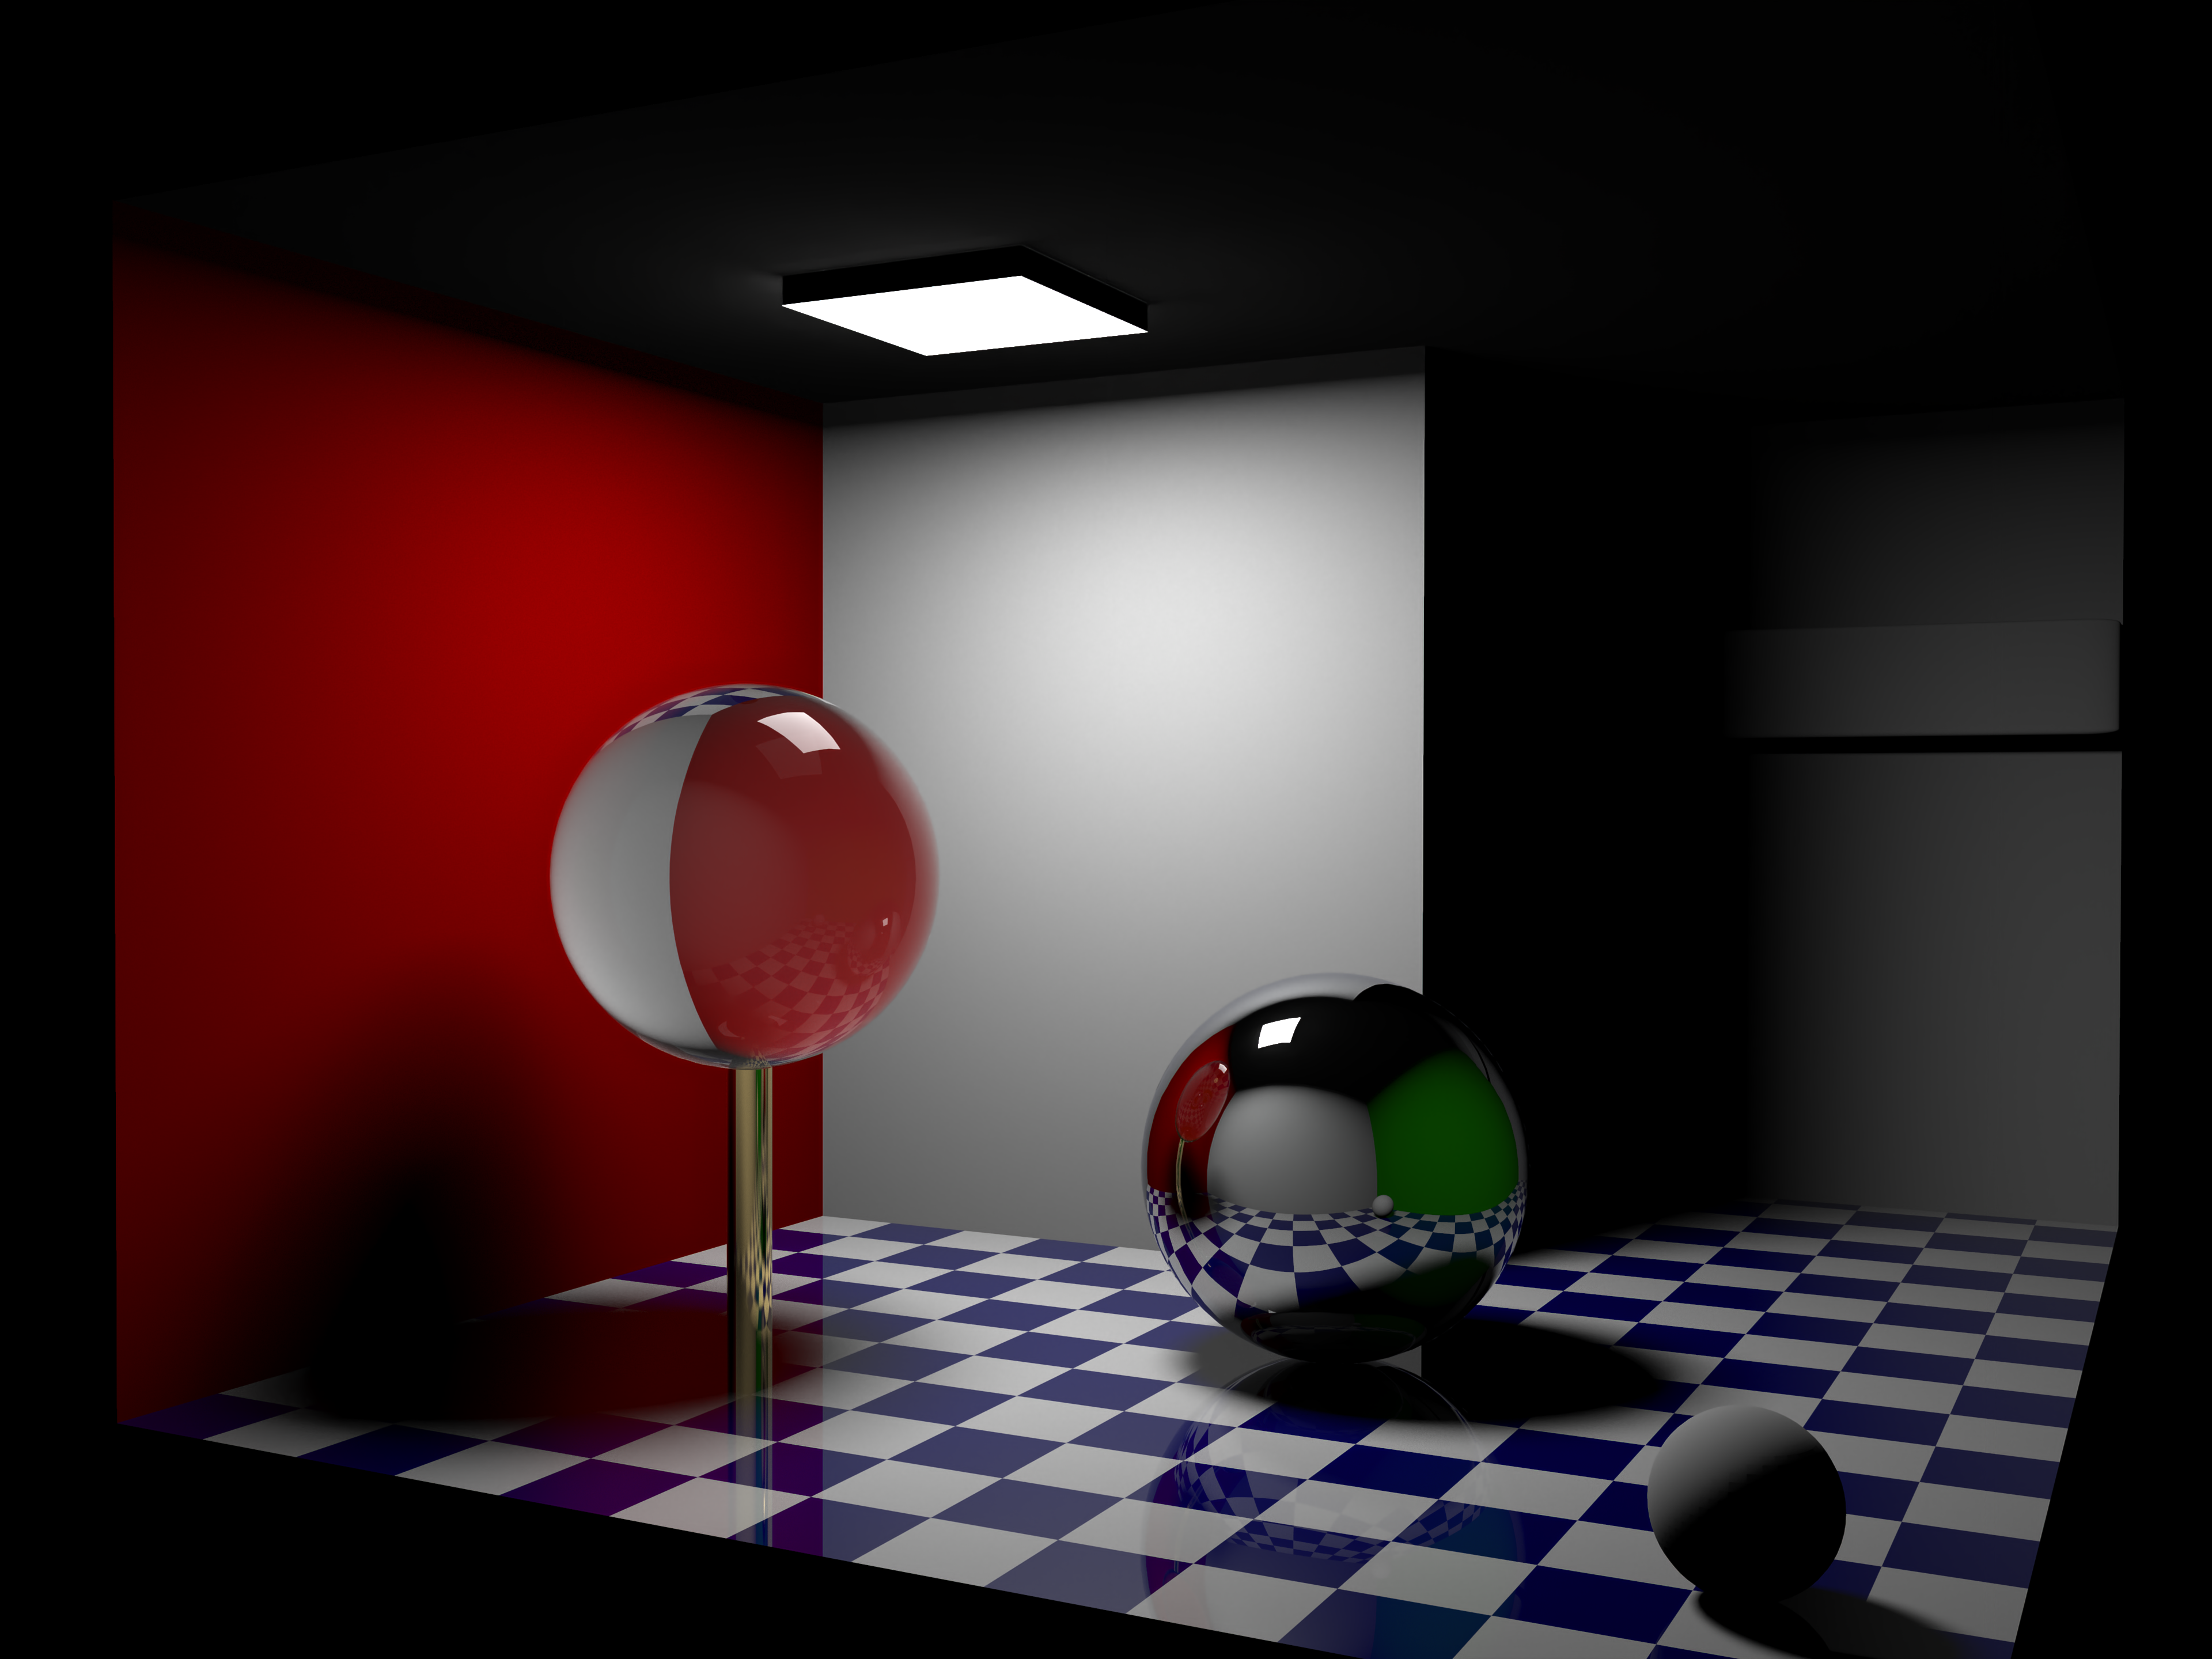
\includegraphics[scale=0.65]{Graphics/Direct_lighting.png}
		\caption{Scene lighting with direct illumination only. By Barahag - Own work, CC BY-SA 4.0}
		\url{https://commons.wikimedia.org/w/index.php?curid=88541991}
		\label{Direct Illumination}
	\end{minipage}\hfill
	\begin{minipage}{0.48\textwidth}
		\centering
		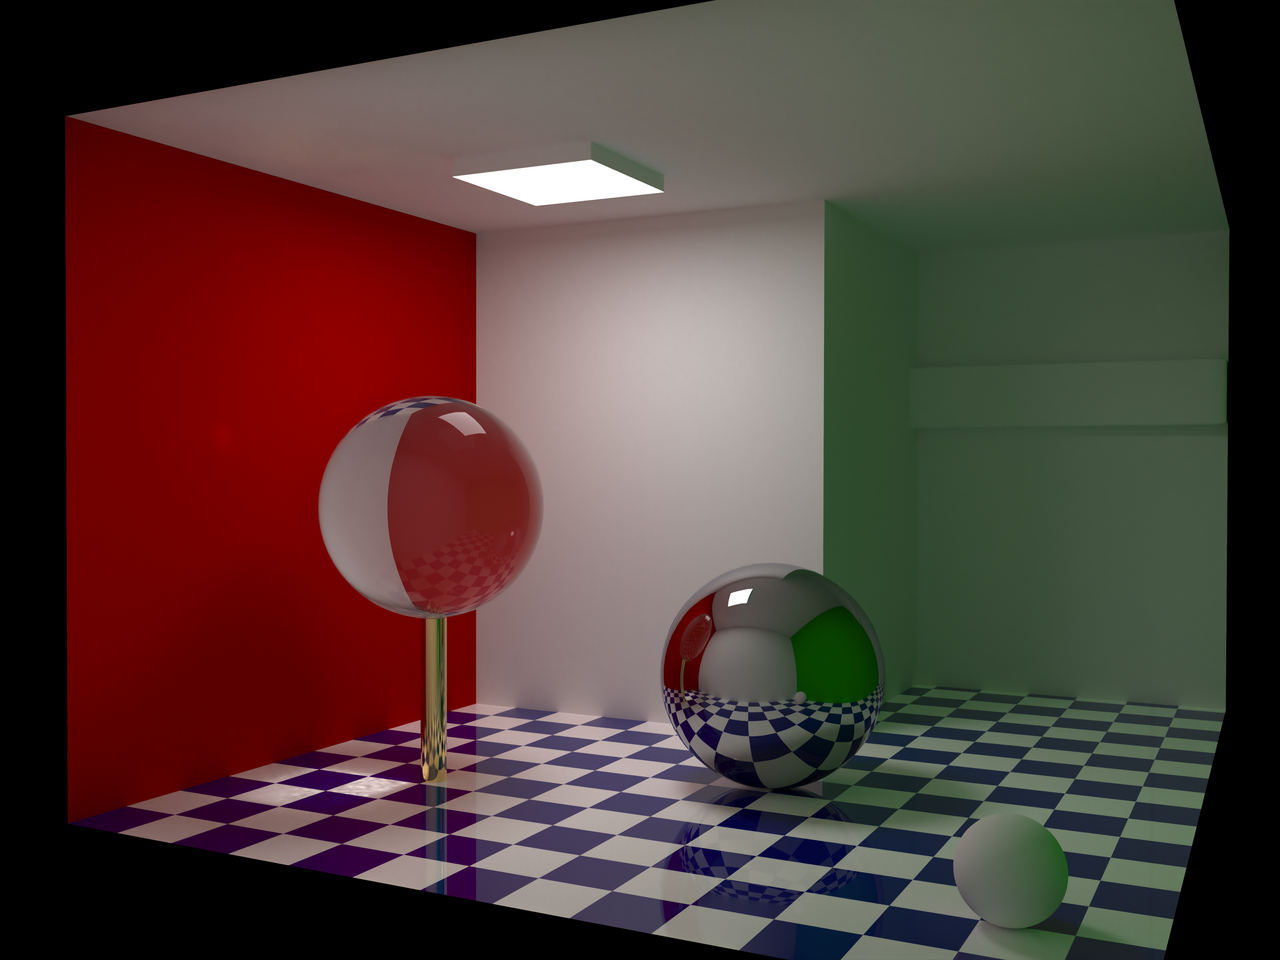
\includegraphics[scale=0.65]{Graphics/Global_illumination.png}
		\caption{Scene lighting with Global illumination. By Barahag - Own work, CC BY-SA 4.0}
		\url{https://commons.wikimedia.org/w/index.php?curid=88540888}
		\label{Global Illumination}
	\end{minipage}
\end{figure}

The field-standard for accurate lighting and shadows in a scene is Path-Tracing, a method that tracks every light ray and any interactions it has with the objects of a 3D scene and calculates the resulting color for each pixel of the screen. Such approach remains prohibitively expensive for most interactive applications, so real-time systems employ precomputation and approximation of the illumination of the scene; static geometry is baked into lightmaps that store per-texel irradiance, while dynamic elements sample from irradiance volumes or light probes, sparse 3D points whose spherical-harmonic coefficients are interpolated at runtime. 

Screen-space GI methods typically approximate a limited number of light-ray bounces directly from the camera's depth buffer, but suffer from missing contextual information outside the camera's view frustum and temporal instability. Voxel-based approaches (e.g., cone-tracing through a low resolution 3D grid) % citation?
enable more dynamic multi-bounce effects at the cost of memory, processing cost and potential blurring of fine detail. 

Across all these techniques, the central challenge is allocating a strict millisecond-scale budget to indirect illumination while maintaining consistency across static and dynamic scene content, avoiding visible seams when blending baked and runtime solutions and fitting within GPU memory constraints. 

Light probes, in particular, represent a compelling middle-ground, flexible enough to illuminate moving objects without rebaking yet compact enough for real-time evaluation, making their optimal placement a critical factor in any high-quality GI pipeline.

% citations where needed?
% fix typos if any, better wording at 1 and 2 paragraph?

%\pagebreak % temporary potentially	

\section{Related Work}
There is an abundance of work in the literature addressing the problem of Global Illumination. These studies aim to achieve realistic lighting in 3D scenes by employing various approaches and techniques, each offering unique advantages and disadvantages, but they share a common goal: to maximize visual fidelity while minimizing computational costs.

\subsection{Offline Methods}
Offline Illumination methods refer to techniques that are not viable for real-time applications and are therefore used only in situations where the importance of high visual fidelity far outweighs the need for computational speed, typically in non-interactive 3D renders, most commonly in movies or pre-rendered scenes. Classic Path-Tracing, first introduced in 1986 \parencite{Kajiya1986}, tracks the movement of a photon ray emitted from a source, typically the camera, and simulates physics interactions to calculate the color of each screen pixel accurately. The immense computational cost of path-tracing led to the development of performance improvements, such as the Metropolis Light Transport (MLT) method introduced in 1997 \parencite{Veach1997}, and variants like bi-directional Path-Trace \parencite{Lafortune1993}, which build on Monte-Carlo algorithms \parencite{Lafortune1996}.

\subsection{Online Methods} % maybe section these?
In contrast, online methods aim to calculate GI interactions in real-time, most commonly used in interactive applications like video games or simulations. They try to balance performance and accuracy, a task that is often difficult due to the processing cost of the calculations for a realistic result. Therefore, these methods take shortcuts, either approximating the GI interactions to a certain degree to maintain framerate budgets, or by precomputing some of the data, wherever possible.

\subsection*{Traditional Methods} % rename this to something better
Techniques that precompute the illumination of a scene only do so for static geometry; objects in the scene that will never change their position, rotation or scale. The algorithms "bake" the required information onto texture maps, which are rendered as such when needed. Light-mapping is one such technique. It precomputes surface brightness and has a low runtime cost. The game Quake was the first interactive application that used lightmaps for rendering GI \parencite{WikiLightmaps}.

Another early technique is the Irradiance Volumes algorithm  \parencite{Greger1998}, which scatters spherical-harmonic (SH) irradiance samples on a 3D grid on the scene. At runtime, lighting is interpolated from the nearest SH cells; this underlies many probe systems, like Unity's light-probe system that implicitly implements a sparse irradiance volume.

More recent static-GI algorithms include Light Field Probes \parencite{McGuire2017}. Light Field Probes extend standard irradiance probes by additionally storing per-texel visibility for each probe. Furthermore, \cite{Xu2022} introduce Discrete Visibility Fields for static ray-traced lighting. The method precomputes occlusion masks stored in a uniform voxel grid, and at runtime, rays that hit a cell use the stored precomputed masks to quickly cull visibility, skipping geometry already known to be occluded.

Unity's new Adaptive Probe Volumes (APV) build on irradiance volumes by automatically populating a grid, with density matched to local geometry. APV then performs per-pixel probe sampling; each pixel blends from the eight nearest probes \parencite{Unity2025}.

Additionally, there are methods that don't focus on Probes for GI. A prevalent example is Unreal Engine's Lumen, a dynamic GI and reflections system that uses a hybrid tracing approach; It starts with a cheap screen-space or signed-distance-field ray cast, and then falls back to more expensive methods like hardware ray tracing \parencite{Unreal2025}.

NVIDIA has also developed RTXGI, a GPU-accelerated library implementing Dynamic Diffuse GI, using a volumetric grid of irradiance probes, which update every frame using hardware-accelerated ray tracing, creating accurate results at the cost of hardware-restricted algorithms and a relatively escalated cost of calculation \parencite{Nvidia2024}.

\cite{Crassin2011} introduced Voxel Cone Tracing (VCT) to approximate real-time GI. In VCT, the scene's static geometry and lighting are "voxelized" into a 3D texture with multiple levels of mipmapping, containing radiance and opacity. At runtime, indirect illumination is approximated by tracing a few low-resolution "cones" from each surface sample into the aforementioned voxel grid, summing the values from regions of voxels.\newline

Even though there are numerous methods trying to solve real-time GI issues, a big percentage of them tend to revolve around probes of various types; most commonly calculating irradiance values among other high-importance metrics. Therefore, it is vital for a 3D scene to have proper probe placement for best results. There are a few methods that try to automate that process, often by placing the probes in a regular grid and only removing the probes that are inside objects, but that can lead to over-sampling, leading to performance costs, mainly in memory usage budgets. Furthermore, some techniques try to remove additional probes using heuristic methods, therefore approaching optimal placement, but with a significant precomputational cost.

\cite{Wang2019} introduce an automatic non-uniform placing scheme using 3D scene skeletons and gradient-descent refinement to cover important locations without redundant probes. A very recent work by \cite{Teuber2024} formulates geometry-based optimization of probe placement using various mesh features, to further improve the lighting in VR/AR scenarios.

Similarly, \cite{Vardis2021} approach the problem by starting with a probe set on a dense grid and iteratively removing the least-important probes using radiance error tests, preserving the global light field while minimizing probe count.

\subsection*{AI-based Methods}
Recently, AI-assisted methods have started to be developed in order to improve GI in 3D applications, specifically in probe-based solutions. \cite{Guo2022} propose a hybrid neural probe GI. They use a gradient-based search to re-project stored probe radiance for any view, therefore eliminating parallax, and then apply a small neural network to reconstruct high-quality images from low-resolution probe data. Related, \cite{You2024} created Neural Light Field Probes, which works by decomposing a scene into a grid of trainable light field probes. Each of these probes encodes local radiance and visibility in a compact feature map. Finally, a neural network optimizes these probes so that the summation of their contributions reproduces the full scene lighting. 

\section{Thesis Structure} % redo parts of this, fix stuff
The structure of the remainder of this thesis will be described shortly. Chapter 2, titled IDK YET, FIX IT, covers important information about light probes and their implementation, describes the AI model basis that was used for our implementation, and introduces the tools and technologies that were used in this thesis. Chapter 3, titled Our Approach (?), presents our method, describes the implementation of the algorithms used, and explains how each part is combined to create the Light-Probe Neural Network (LPNN), our neural network system that attempts to speed up light probe placement in Unity 3D scenes by predicting importance values for the given grid set and placing only the most vital light probes, affected by a user-controlled threshold value. Each grid position gathers samples of a few metrics, which are then used by the neural network to decide whether or not it is vital to place a light probe in each individual cell of the 3D grid. A step-by-step process of creating the grid, getting the features out of the grid cells, and placing the probes and baking the global illumination inside Unity. Additionally, the feature set can be used to retrain the AI model, we explain how to create the labels needed for the process, and how to import the new model to Unity using Sentis for usage. Chapter 4, titled Experiments, presents an experimental comparative and qualitative evaluation between the proposed method and some of the already introduced algorithms. Finally, Chapter 5, titled Conclusions and Future Works, concludes the thesis and proposes directions for future work based on this thesis.













	
	\chapter{Review of the Literature}
	theoretical background, what light probes are, technologies used

\section{Light Probes}
TODO

	
	\chapter{Our Approach}
	In this chapter, we will present the pipeline of the tool and its implementation. The chapter will be split into five parts, describing the process of collecting the features, how labels are created, LPNN training in python, and predicting light probe positions using the trained model accordingly. Lastly, we will present the tool inside the Unity Editor.

\section{Feature Collection}
A necessary step before collecting scene and lighting features is to first place points in the scene to collect data per-point. We decided to create an algorithm that places those points, called Evaluation Points (EP) henceforth, inside a collection of user-defined potentially concave scene bounds of arbitrary shape. As shown in algorithm \ref{alg:grid_place}, we begin by placing the Evaluation Points on a volume that surrounds the collection of bounds the user defined, then we remove the points that are not within the bounds, as seen in figure \ref{fig:grid}.


\begin{algorithm}
	\caption{Placement of Evaluation Points on a grid-like layout}
	\label{alg:grid_place}
	\begin{algorithmic}[1]
		\Require $cellsize > 0$
		\State $EP = \emptyset$
		\ForAll{$points \in volume$}
			\If{$point \in bounds$}
				\State $EP \gets EP + point$ \Comment add point to the set
			\EndIf
		\EndFor
		\State \Return $EP$
	\end{algorithmic}
\end{algorithm}

In algorithm \ref{alg:grid_place}, \textit{cellsize} is the distance between each EP, and a value of 0 or negative values do not apply, therefore it is vital to require a \textit{cellsize} bigger than 0. \textit{Cellsize} is not directly shown inside the algorithm, but for the C\# implementation it is necessary and the value is used often, therefore we show the requirement here. \textit{Bounds} is the collection of 3D areas defined by the user, and \textit{volume} are the bounds of that collection. As seen in figure \ref{fig:grid}, the rectangles shown in pink are three distinct areas defined by the user, defining where they want EP placed. Seen in red is the surrounding volumes of those bounds. We clearly see the EP, shown as yellow dots. They are present only inside the areas of the user defined bounds, but in a grid layout, regardless of the position of those bounds. The EP intentionally "overshoot" the bounds for completeness when calculating the feature data for each point, making sure we cover the entirety of the bounds given by the user.

\begin{figure}[h]
	\centering
	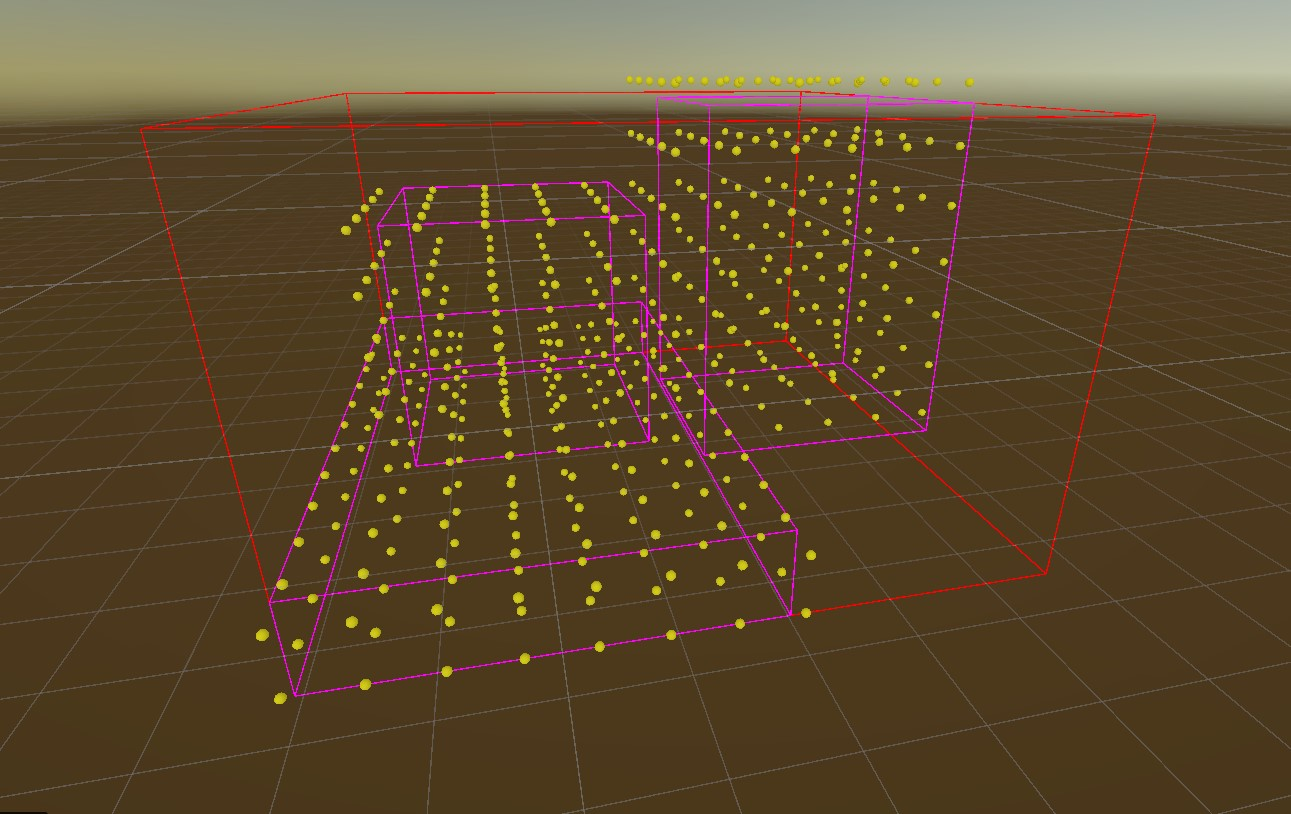
\includegraphics[scale=0.43]{Graphics/Grid_Example.jpg}
	\caption{A 3D Scene showing the placement of Evaluation Points (shown in yellow) inside the user defined bounds (shown in pink), contained within the calculated volume (shown in red).}
	\label{fig:grid}
\end{figure}

After placing the EP, we use each point to calculate the data needed for the feature vectors. The aim of the LPNN model is to give an importance value to each of those EP that it is given. Therefore, it is vital that it understands what defines a significant point via the features that it is trained on. Our knowledge dictates that an important location for a light probe is one that has great variance in illumination. Therefore, we include light-, RGB- and normal-variance as features for each point. Light-Variance dictates how much the light intensity changes around a point. RGB-Variance is similar, since it shows the change in Red, Green, and Blue light around each point, each channel being independent from the others. Normal-Variance is a value that makes locations like corners distinct from empty areas or from locations near a wall. Similarly, we also calculate Occlusion-Factor, a feature that gives each point a value depending on how empty or cluttered the area around it is. Normal-Variance together with Occlusion-Factor inform the model of areas that are enclosed or close to complex geometry. This makes the model able to distinguish these locations, even when all other values are identical, making it able to give different importance values to those distinct locations.

Along with the features mentioned above, we additionally include a vector that contains the spherical-harmonic values for a small amount of distinct directions around each point. The implementations of each feature collection method are shown in \ref{alg:feat_sh}, \ref{alg:feat_lv}, \ref{alg:feat_rgbv}, \ref{alg:feat_nv}, and \ref{alg:feat_of}.


\begin{algorithm}
	\caption{Feature Extraction: Spherical Harmonics around a point}
	\label{alg:feat_sh}
	\begin{algorithmic}[1]
		\Require $EP \neq \emptyset$
		\State $values = \emptyset$
		\ForAll{$points \in EP$}
			\State $value \gets evaluateSH(point)$
			\State $values \gets values + value$ \Comment add SH to the list
		\EndFor
		\State \Return $values$
	\end{algorithmic}
\end{algorithm}

\begin{algorithm}
	\caption{Feature Extraction: Light Variance around a point}
	\label{alg:feat_lv}
	\begin{algorithmic}[1]
		\Require $EP \neq \emptyset$
		\Require $samples \geq 1$ \Comment The amount of directions
		\State $radius \gets 1$ \Comment How far around the point to check
		\ForAll{$points \in EP$}
			\State $luminances = \emptyset$
			\For{$n = 1,\dots,samples$}
				\State $direction \gets$ random point on sphere with $radius$
				\State $sh \gets evaluateSH(direction)$
				\State $luminance \gets sh.R * 0.2126 + sh.G * 0.7152 + sh.B * 0.0722$ \Comment From RGB to luminance value
				\label{alg:feat_lv:7}
				\State $luminances \gets luminances + luminance$ \Comment Add luminance to the list
			\EndFor
			\State $mean \gets mean(luminances)$ \Comment Get the mean value of the luminances
			\State $variance \gets (luminances - mean)^2 \div samples$ \Comment Get the total variance of luminances
		\EndFor
		\State \Return $variance$ per point
	\end{algorithmic}
\end{algorithm}

In line \algref{alg:feat_lv}{alg:feat_lv:7}, to convert from RGB channel values to perceived light intensity of the pixel, also known as luminance, we use the formula shown in \cite{Luminance2015}, under section 3 item 3.2. This formula is used to calculate how bright a pixel in regards to the RGB channel values it currently shows.

\begin{algorithm}
	\caption{Feature Extraction: RGB Variance around a point}
	\label{alg:feat_rgbv}
	\begin{algorithmic}[1]
		\Require $EP \neq \emptyset$
		\Require $samples \geq 1$ \Comment The amount of directions
		\State $radius \gets 10$ \Comment How far around the point to check
		\ForAll{$points \in EP$}
		\State $count \gets 0$
		\For{$n = 1,\dots,samples$}
		\State $direction \gets$ random point on sphere with $radius$
		\State $sh \gets evaluateSH(direction)$
		\EndFor
		\State $meanRGB \gets mean(sh.RGB)$
		\State $RGBvariance \gets (sh.RGB - meanRGB)^2 \div samples$
		\EndFor
		\State \Return ${RGBvariance.R, RGBvariance.G, RGBvariance.B}$ per point
	\end{algorithmic}
\end{algorithm}

\begin{algorithm}
	\caption{Feature Extraction: Normal Variance around a point}
	\label{alg:feat_nv}
	\begin{algorithmic}[1]
		\Require $EP \neq \emptyset$
		\Require $samples \geq 1$ \Comment The amount of directions
		\State $radius \gets 1$ \Comment How far around the point to check
		\ForAll{$points \in EP$}
			\State $normals = \emptyset$
			\For{$n = 1,\dots,samples$}
				\State $direction \gets$ random point on sphere with $radius$
				\State $hit \gets castRay(direction)$
				\If{$hit == True$}
					\State $normals \gets normals + hit.normal$
				\EndIf
			\EndFor
			\State $mean \gets mean(normals)$ \Comment Get the mean direction of the normals
			\State $variance \gets (1- dot(normals, mean)) \div samples$
			\label{alg:feat_nv:12}
			\Comment Get the total variance of normals
		\EndFor
		\State \Return $variance$ per point
	\end{algorithmic}
\end{algorithm}

In line \algref{alg:feat_nv}{alg:feat_nv:12}, we want the higher values to define the areas with more complex geometry. The dot product of vectors is a value between 0 and 1, therefore we subtract the dot product from 1, to invert the range of the variance.

\begin{algorithm}
	\caption{Feature Extraction: Occlusion Factor around a point}
	\label{alg:feat_of}
	\begin{algorithmic}[1]
		\Require $EP \neq \emptyset$
		\Require $samples \geq 1$ \Comment The amount of directions
		\State $radius \gets 10$ \Comment How far around the point to check
		\ForAll{$points \in EP$}
			\State $count \gets 0$
			\For{$n = 1,\dots,samples$}
				\State $direction \gets$ random point on sphere with $radius$
				\State $hit \gets castRay(direction)$
				\If{$hit == True$}
					\State $count \gets count + 1$
				\EndIf
			\EndFor
			\State $factor \gets count \div samples$
			\Comment Percentage of hits versus misses.
		\EndFor
		\State \Return $factor$ per point
	\end{algorithmic}
\end{algorithm}

After collecting all the features, we compact them into a feature vector per-EP, and save them into a file for later use. As shown in \ref{sec:LPNN_UI}, it is also possible to collect feature vectors from multiple scenes at different times, as well as labels, to make the model more accurate by providing more input data. 

\section{Label Collection}

The supervised-learning approach we decided on for this thesis requires that the model also receives labels as an input. Labels are values for each of the input feature vectors that describe the correct output for that feature vector. It is therefore vital to collect labels for each EP that we have also collected features for. For this purpose, we use LumiProbes \parencite{Vardis2021} to collect labels by returning a True or False value, depending on if the cell of each Evaluation Point contains a probe placed by LumiProbes. The use of LumiProbes as the ground-truth was arbitrary. The system is constructed in a way that allows any method of ground-truth light probe placement to be used for label extraction, even manual placement. In algorithm \ref{alg:labels} we check every EP with every light probe in the ground-truth list and set the label to True if there exists a light probe around a \textit{cellsize} radius of that Evaluation Point.

\begin{algorithm}
	\caption{Label Extraction per-EP}
	\label{alg:labels}
	\begin{algorithmic}[1]
		\Require $EP \neq \emptyset$
		\Require $cellsize > 0$
		\ForAll{$points \in EP$}
			\ForAll{$probes \in groundTruth$}
				\If{$probe \in cellsize$ around $point$}
					\State $label \gets True$
				\Else
					\State $label \gets False$
				\EndIf
			\EndFor
		\EndFor
		\State \Return $labels$ per point
	\end{algorithmic}
\end{algorithm}

The nature of this label extraction method beckons for the ground-truth light probe placement to be close to the optimal placement, determined by the user's intuition, experience, and demands for the specific scene.

After collecting the labels into a list, they are saved into a file on the hard disk for use in training of the model, as seen in section \ref{sec:model_training}. As mentioned previously, it is possible to collect labels from multiple scenes, creating a bigger dataset for the model to train on.

\section{Model Training}
\label{sec:model_training}

The model basis for LPNN, as mentioned previously, was a PointNet architecture \parencite{PointNet2017} as described in \ref{sec:background:pointnet}.

\section{Light Probe Prediction}

\section{LPNN inside Unity Editor}
\label{sec:LPNN_UI}

	
	\chapter{Experiments}
	In this chapter, we present experimental results of the LPNN approach. The evaluation is qualitative, since the nature of light probes and their optimal placement is subjective to the user and the needs of the application. We focus mainly on speed in relation to light probe layout given by the tool. We compare performance results to LumiProbes \parencite{Vardis2021}. All experiments were conducted in Unity 6 version 6000.0.38f1, on a system comprising of an NVIDIA RTX2060M GPU, 16GB DDR4 RAM and an Intel i7-9750H CPU, on a Windows 10 Operating System.

\section{Performance}
\label{sec:4_performance}
Since the focus of the thesis was to speed up the placement of light probes in this stage of any 3D application development iteration process, we will focus on the execution time of the tool and also critique the results and their qualitative properties, to make sure the placements are correct. Indeed, as seen in table \ref{table:times}, the LPNN approach speeds up light probe placement by orders of magnitude faster than other approaches, but it may suffer from occasional misplacement; probes that were placed in positions that are not vital, leading to oversampling, which we will show shortly. In experiments where LumiProbes and LPNN were requested to place close to the same amount of light probes in the same scene, LPNN time stayed close to constant, typically up to a few seconds, regardless of the scenario or the amount requested. Results for various amounts of light probes and scenes are presented in table \ref{table:times}. Times are averaged over multiple runs. Units are represented in minutes (m), seconds (s), or milliseconds (ms). Where applicable, we also append the settings used for each tool. For LumiProbes, settings include the grid parameters and the evaluation-point count. All other settings are as follows: Evaluation point placement type is set to Poisson, Decimation type is set to Medium, Decimation directions are averaged, Decimation metric is set to  Chrominance, Minimum LP set is disabled, and Maximum Error is set to 3. For LPNN, settings include the threshold value used for the specific result and the cell size of the 3D grid, in order. Figures for the results are shown in section \ref{sec:4_quality}. Memory requirements for this tool are strictly dependent on the amount of light probes present in the scene, since all information needed by the tool are either already present in Unity and are needed regardless of the presence of the tool, e.g. Global Illumination data, or are stored on the Hard Disk of the system as files with storage sizes dependent on the amount of probes placed before the execution of the tool. File sizes for 150 probes were less than 2KB. Typically, the tool creates files needed for placing the light probes with size-scaling 1KB per approximately 100 probes.

\begin{table}
	\centering
\begin{tabular}{ |c||c|c|c|c|c|  }
	\hline
	\multicolumn{6}{|c|}{Execution time} \\
	\hline
	Method & Scene & Time & P. Count & P. Present (\& Removed) & Settings\\
	\hline
	LumiProbes & Sponza   & 22.443s  & 105 & 34 (75)  & (7,3,5), 128 \\
	\cline{2-6}
	           & Office   & 51.059s  & 144 & 84 (60)  & (12,3,4), 128\\
	           &          & 919.134s & 288 & 182 (106)& (12,3,8), 256\\
	\cline{2-6}
	           & Corridor & 161.151s & 180 & 120 (60) & (20,3,3), 256\\
	           &          & 477.648s & 243 & 147 (96) & (27,3,3), 256\\
	\hline
	\hline
	Ours       & Sponza   & \textbf{5.3ms}  & 90  & 54 (36)   & 0.4, 2.0 \\
			   &          & \textbf{17.8ms} & 400 & 40 (360)  & 0.9, 1.3 \\
	\cline{2-6}
			   & Office   & \textbf{7.8ms}  & 140 & 34 (106)  & 0.758, 1.87 \\
               &          & \textbf{25.2ms} & 832 & 117 (715) & 0.859, 1.10 \\
    \cline{2-6}
    		   & Corridor & \textbf{10.9ms} & 186 & 84 (102)  & 0.549, 1.94 \\
               &          & \textbf{15.7ms} & 246 & 95 (151)  & 0.615, 1.50 \\
               
	\hline
\end{tabular}
\caption{Execution time for LPNN and LumiProbes on a select number of scenes and probe counts. \textit{P. count} represents the total amount of probes in the scene, before simplification. \textit{P. Present} depict the final amount of probes after running the tools. The number in parenthesis is the amount of probes removed by the tool, in respect to the settings. Fastest times are shown in \textbf{bold}.}
\label{table:times}
\end{table}

\section{Quality}
\label{sec:4_quality}
The tools were tested on the aforementioned edited Sponza scene \parencite{Sponza2017}, Corridor scene \parencite{Corridor2021} and Office scene \parencite{Office2021}. We will present the qualitative results. As we will see shortly, LPNN correctly places light probes in areas of high variance.

\begin{figure}[h]
	\centering
	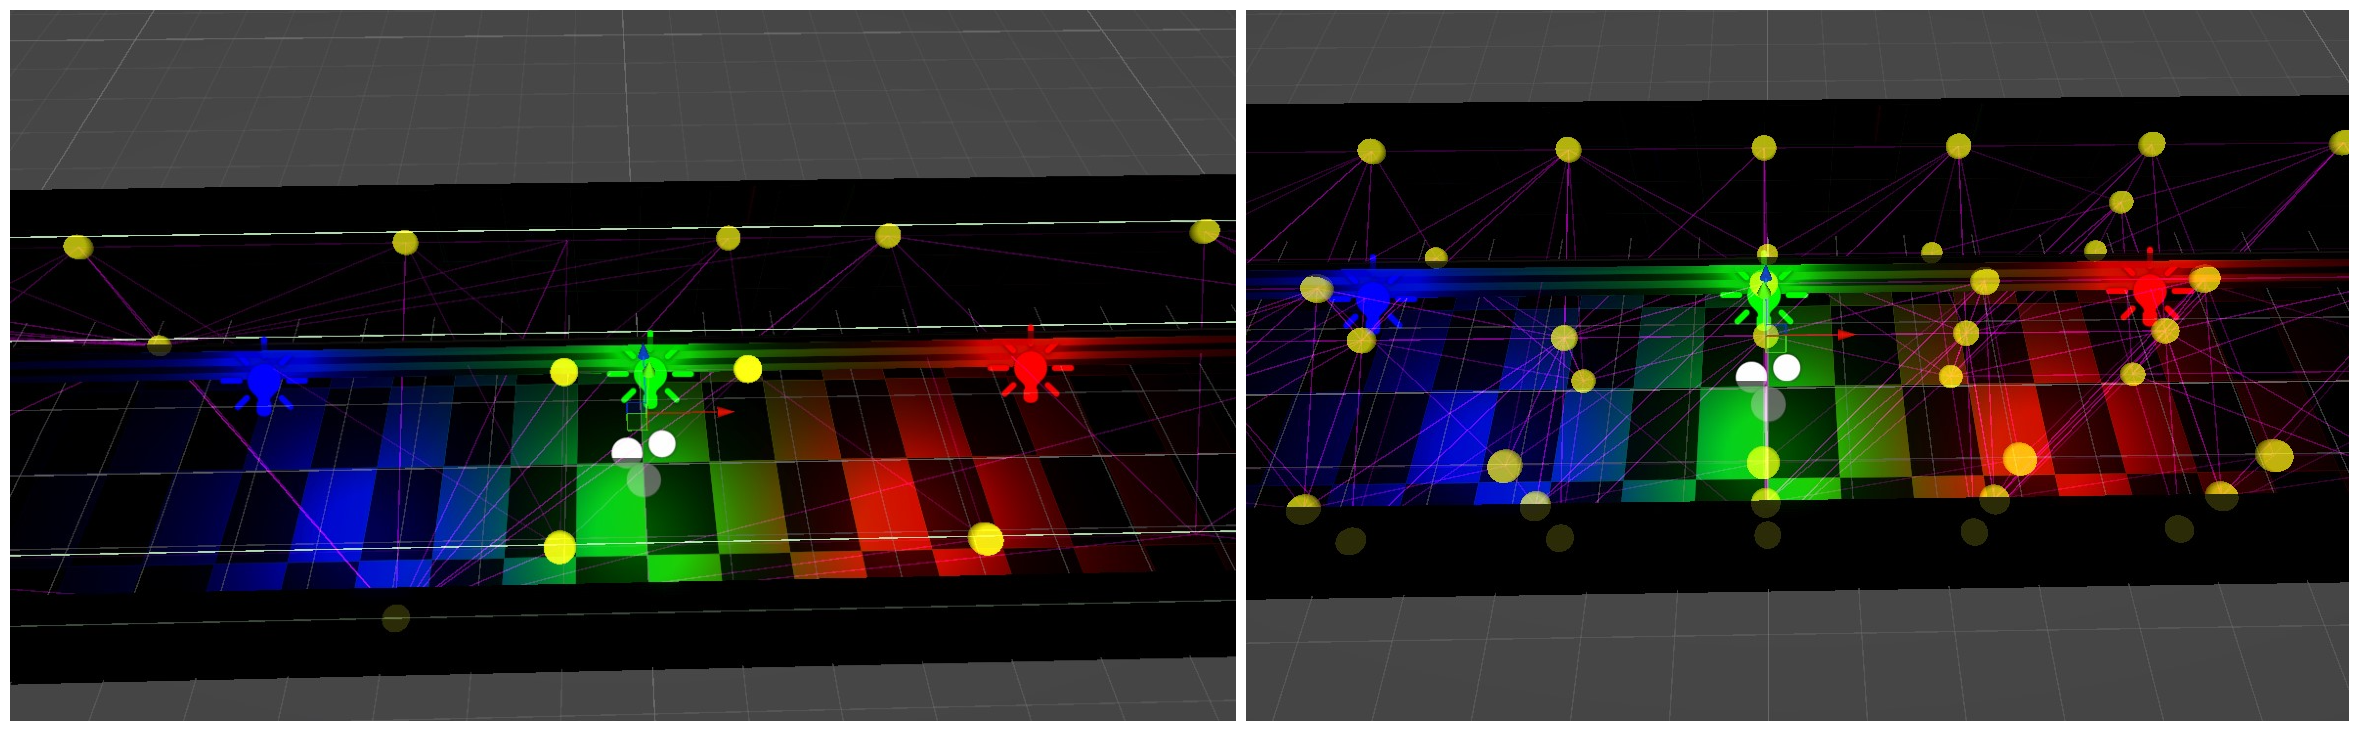
\includegraphics[scale=0.18]{Graphics/results/concats/comparison1.png}
	\caption{A 3D Scene showing a comparison of light probe placement in a \textbf{high} color-variance scenario, between LPNN (left) and LumiProbes (right) with settings 0.549, 1.94 and (27,3,3), 256 respectively, in the Corridor scene.}
	\label{fig:comp1}
\end{figure}

As shown in figure \ref{fig:comp1}, we can clearly see that the LPNN tool has correctly placed light probes between the blue and green light sources, as well as between the green and red light sources, locations with great variance in Chrominance, It has additionally kept the amount of probes at a minimum, only placing one probe at each location mentioned. This result is close to optimal placement, since the distance between the light sources is only 4 units, making additional probes unnecessary in most scenarios. It should be noted that the tool did correctly place probes on the edges of the bounds, seen as light-green colored lines. This ensures that any dynamic object that moves outside the bounds set by the user continues to have some light-probes information for its illumination. 

\begin{figure}[h]
	\centering
	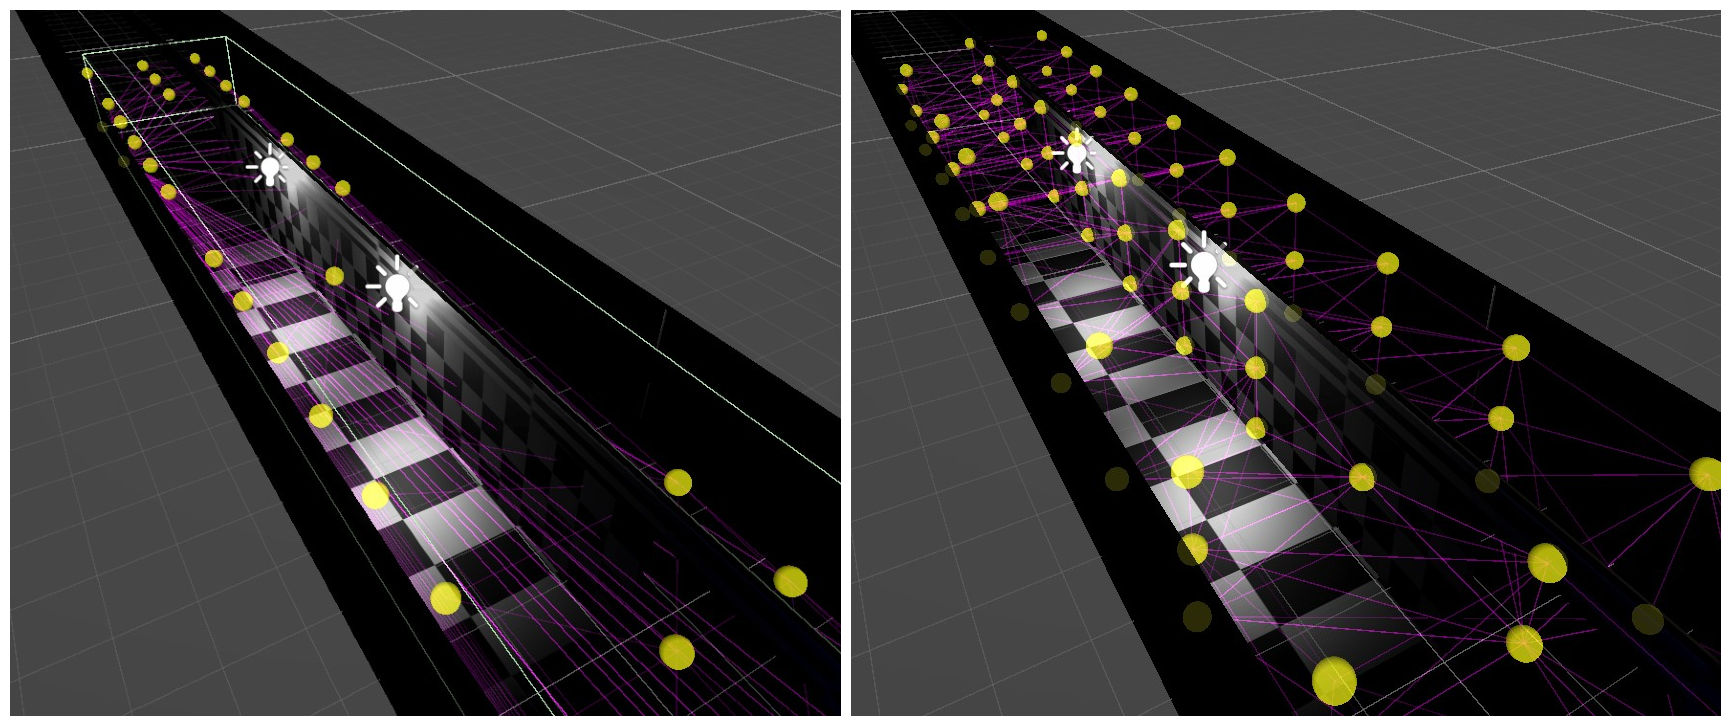
\includegraphics[scale=0.25]{Graphics/results/concats/comparison2.png}
	\caption{A 3D Scene showing a comparison of light probe placement in a \textbf{low} color-variance scenario, between LPNN (left) and LumiProbes (right) with settings 0.615, 1.5 and (27,3,3), 256 respectively, in the Corridor scene.}
	\label{fig:comp2}
\end{figure}


	
	\chapter{Conclusions and Future Work}
	In this thesis, the LPNN method is implemented to accelerate the placement of light probes in a 3D scene during the development process. The method is experimented on, and the results are presented. The LPNN method and its normal usage are described. Additionally, the process of collecting the required features and labels needed for retraining the Neural Network is also presented. This approach assigns an importance score to a grid-like layout of Evaluation Points, which are then used to place light probes in the scene, depending on a variable threshold value controlled by the developer. Finally, quantitative and qualitative results are presented. 

In the experiments conducted, we concluded that the Neural Network approach is capable of reducing the time needed by the developer for a sufficient light probe layout, as well as minimizing the amount of manual tweaking required for optimal results. The results present a solution that approaches a theoretical optimal light probe layout. While not free of oversampling or undersampling, the LPNN tool provides a consistently suitable layout within a fraction of the time needed by other methods, including the manual approach.

Moving forward from this thesis, an improved Neural Network architecture can be explored, implemented and experimented on. An approach that takes into consideration the edges of each light probe can potentially improve the accuracy of the model presented. While a Deep Learning approach requires a large dataset to be able to generalize sufficiently, an improved architecture and implementation can reduce the cost and improve accuracy by providing more variety in the training data. Additionally, a heuristic approach can be combined, removing or adding light probes in areas that the model inferred to be of low-significance, allowing for results closer to the theoretical optimal layout. Lastly, a new approach can be explored that combines the LPNN approach with the Neural Light Field Probes method \parencite{You2024}, ensuring that the contributions of both methods are preserved.
	
	% at the end
	\setlength\bibitemsep{2\itemsep}
	\printbibliography

	

	
\end{document}